% RASD — Ring Attention with Speculative Decoding for Million-Token Inference
% arXiv preprint, NeurIPS 2026 preprint style.
%
% Build: cd manuscript/arxiv && pdflatex main && bibtex main && pdflatex main && pdflatex main
%
% Source data is committed in the repo:
%   tables/main_*.tex        — auto-generated, via scripts/emit_main_tables.py
%   figures/fig*.pdf         — auto-generated, via scripts/plot_figure*.py
%   results/final/final_results.json — single canonical aggregate

\documentclass[11pt]{article}

% NOTE: NeurIPS 2026 style file (neurips_2026.sty) drops in for the
% camera-ready submission. For local review / arXiv we use a vanilla
% article class with NeurIPS-like geometry; the page count differs
% by ~10% but content is unchanged.
%   \usepackage[preprint]{neurips_2026}
\usepackage[a4paper,margin=1in,textheight=9.5in]{geometry}

% --- Packages -------------------------------------------------------------
\usepackage[utf8]{inputenc}
\usepackage[T1]{fontenc}
\usepackage[hidelinks]{hyperref}
\usepackage{url}
\usepackage{booktabs}
\usepackage{amsfonts}
\usepackage{amsmath}
\usepackage{amssymb}
\usepackage{textcomp}
\usepackage{nicefrac}
\usepackage{microtype}
\usepackage{xcolor}
\usepackage{graphicx}
\usepackage{subcaption}
\usepackage{enumitem}
\usepackage{authblk}        % \author + \affil
\usepackage{natbib}         % \citep / \citet
\usepackage{array}          % \arraybackslash + >{...} column modifiers
\usepackage{tikz}           % architecture diagram
\usetikzlibrary{positioning,arrows.meta,calc,shapes.geometric,fit,backgrounds}
% \url package's \path is a breakable \texttt — use for long file paths,
% revision hashes, and identifiers that don't fit on one line.
% Already loaded via \usepackage{url} above.
\urlstyle{tt}               % \url / \path render in typewriter font
\Urlmuskip=0mu plus 1mu     % allow breaks at any char (not just /)
% Softer than \sloppy: lets TeX stretch up to 3em as a last resort
% to avoid Overfull \hbox warnings on paragraphs that contain long
% unbreakable \path / \texttt tokens. Avoids the ugly large gaps
% \sloppy produces in normal paragraphs.
\emergencystretch=3em
% Cyrillic characters appear in one qualitative-table excerpt
% (rendered garbage from YaRN-degraded generation); guard against
% compile errors:
\providecommand{\cyrtext}[1]{\textbf{[Cyrillic]}}

\graphicspath{{../../figures/}{./}}

% --- Title block ----------------------------------------------------------
\title{When Speculative Decoding Stops Paying Off at Long Context:\\
       A Diagnostic Study with RASD}

\author[1]{Aman Kesarwani\thanks{\texttt{amankesarwani@berkeley.edu}}}
\author[2]{Raj Dandekar\thanks{Advisor.}}
\affil[1]{}
\affil[2]{}

\begin{document}
\maketitle

% =========================================================================
% Abstract — seeded from mentor's roadmap + M4 measured findings
% =========================================================================
\begin{abstract}
Speculative decoding amortizes a target-model forward pass into
$\gamma+1$ tokens when a small draft model agrees with the
target, yielding 2--3$\times$ speedups at short context. We ask
whether this speedup transfers to million-token inference and
find it does not. Per-round acceptance becomes bimodal at long
context on Llama-2-7B with YaRN factor 256: about half of verify
rounds fully reject the draft, and the cumulative speedup against
a matched target-only baseline regresses to $0.96\times$ at
512\,k and reaches parity ($1.00\times$) at 1\,M. A
short-context control on real text confirms the bimodality is
base-model behavior under YaRN extrapolation, not an RASD
limitation. A profiler measurement shows communication is
${\leq}1.2\%$ of wall on the speculator rank, ruling out overlap
between speculative work and ring communication as the mechanism
behind the moderate-context speedup. Arriving at these findings
required a system that can actually run a target-model forward at
1\,M context. To that end we built \textbf{RASD} (Ring Attention
with Speculative Decoding), which combines ring-attention
sequence parallelism, NF4 KV-cache quantization (chunked, with a
bf16 attention-sink prefix), YaRN position scaling, and
speculative verification with a small draft model. On
8$\times$A100 80\,GB SXM4, RASD runs Llama-2-7B inference at
1\,M-token context with 40\,GB peak per rank, while vanilla
HuggingFace FlashAttention-2 runs out of memory at 128\,k
single-rank. We derive the dominant terms of the per-rank memory
equation, and show the chunked-NF4 KV update is what brings the
1\,M case inside the per-rank budget. The same three-seed
apples-to-apples matrix that yields parity at 1\,M shows a
1.24--1.80$\times$ speedup at moderate contexts (128\,k--256\,k).
We release the implementation under the MIT license with
version-pinned dependencies, every per-position acceptance
trace, and the full M3 ablation grid that derived the system's
design point.
\end{abstract}

% =========================================================================
% Section 1 — Introduction
% =========================================================================
\section{Introduction}
\label{sec:intro}

Long-context language model inference has emerged as the
rate-limiting step for several practical workloads: multi-document
question answering over book-length corpora, agentic workflows that
accumulate hours of tool-call traces, retrieval-free in-context
learning at the scale of a small library, and analysis of complete
code repositories.  Frontier closed-source systems already advertise
context windows in the millions of tokens.  Reproducing that
capability on commodity, open hardware --- 8 GPUs on a single node,
the configuration available to most academic and small-industry
groups --- requires solving two compounding bottlenecks
simultaneously.

\paragraph{Bottleneck 1 (memory).}
The key-value (KV) cache grows linearly with sequence length.  For
Llama-2-7B in bf16, a 1 million-token KV cache occupies approximately
67\,GB --- already exceeding a single A100 80\,GB --- and the
attention matrix for prefill scales quadratically.  Ring Attention
\citep{liu2023ringattention} resolves this by sharding the sequence
dimension across $W$ ranks and pipelining the per-block attention
computation through a ring of inter-rank exchanges.  Combined with
FlashAttention-2 \citep{dao2023flashattention2} for the local
attention kernel and KV quantization (NF4
\citep{dettmers2023qlora}, KIVI \citep{liu2024kivi},
KVQuant \citep{hooper2024kvquant}) for cache compression, sub-100\,GB
per-rank footprints become feasible at 1\,M context.

\paragraph{Bottleneck 2 (latency).}
Once memory fits, autoregressive decoding remains expensive: each
generated token requires a full forward pass through the model, with
attention costs that grow with the context length already in the
KV cache.  Speculative decoding
\citep{leviathan2023fast,chen2023accelerating,miao2023specinfer,cai2024medusa}
amortizes this cost by having a small draft model propose $k$
tokens, then verifying all $k$ with a single target-model forward
pass and accepting the longest matching prefix.  When the draft and
target agree often (high \emph{acceptance rate} $\alpha$), the
target pays one forward to generate $1 + k\alpha$ tokens.  At
short context, this routinely yields $2\text{--}4\times$ speedups.

\paragraph{The question this paper asks.}
At short context, speculative decoding yields 2--3$\times$
speedups on standard inference benchmarks. We ask whether this
speedup transfers to million-token inference. Answering the
question requires a system that can run a target-model forward at
1\,M context on commodity hardware. Both ring attention and
speculative decoding exist as mature open-source components, but
they have not been combined into a published million-token
inference system. Doing so surfaces practical questions: how does
NF4 KV quantization interact with the YaRN \citep{peng2023yarn}
position scaling required to push Llama-2-7B past its 4\,k
training horizon; how does the speculative verify loop's
broadcast-and-resample pattern compose with the ring attention's
existing collective; and most importantly, \emph{does the
speculative speedup that exists at 4\,k transfer to 1\,M, or do
acceptance rates collapse out of the regime where the technique
is useful?}

\paragraph{The RASD system.}
We present \textbf{RASD} (Ring Attention with Speculative Decoding),
an inference system that combines (i) ring-attention sequence
parallelism, (ii) NF4 KV-cache quantization with chunked updates and
a bf16 outlier-keep prefix \citep{xiao2024streamingllm} on rank 0,
(iii) YaRN position scaling, and (iv) speculative verification with a
1.3\,B-parameter draft model into a single end-to-end loop.  On
8$\times$A100 80\,GB SXM4, RASD runs Llama-2-7B inference at
1\,M context with 40\,GB peak per rank.  In the same hardware
configuration, vanilla HuggingFace FlashAttention-2 \texttt{generate()}
runs out of memory at 128\,k single-rank --- so a direct
\emph{throughput} comparison at long context is meaningless; the
correct comparison is with an apples-to-apples \emph{target-only}
ablation that uses the same ring infrastructure but disables the
speculative loop.

\paragraph{Empirical findings.}
We report the findings up-front so readers can place the rest of
the paper in context. \emph{First}, the answer to the central
question: the speculative speedup at 4\,k does not transfer to
1\,M. The three-seed mean speedup of RASD against a matched
target-only baseline (same RASD infrastructure with the
speculative verify loop disabled) is $1.24\times$ at 128\,k,
$1.80\times$ at 256\,k, regresses to $0.96\times$ at 512\,k, and
reaches parity ($1.00\times$) at 1\,M. \emph{Second}, per-round
acceptance at long context is \emph{bimodal} (about half of
rounds reject the entire draft); a short-context control on real
text shows this bimodality is specific to Llama-2 under YaRN
factor 256 and is not present at the model's native training
context. \emph{Third}, we identify two candidate mechanisms for the
moderate-context speedup: communication-overlap masking (the
original RASD design hypothesis) and draft-phase amortization
of target-model compute. A torch.profiler measurement on the
speculator rank shows communication is $\leq 1.2\%$ of wall
across the matrix; \S\ref{sec:results-profile} interprets this
result in light of both mechanisms. \emph{Fourth}, as a capability result:
on 8$\times$A100 80\,GB SXM4, RASD reaches 1\,M-token context
with a peak per-rank memory of 40\,GB, half the available 80\,GB,
while HuggingFace's standard
\texttt{Llama-2-7b-hf.generate()} with FlashAttention-2 runs out
of memory at 128\,k single-rank, making a direct throughput
comparison at long context not well-defined.

\paragraph{Contributions.}
RASD's central contribution is to amortize the target-model
forward via speculation in a distributed-KV setting; we
characterize when and why this amortization pays off, and when
it does not. Concretely:
\begin{itemize}[leftmargin=*,topsep=0pt]
  \item \textbf{A 1\,M-token inference capability} on 8$\times$A100
        80\,GB at 40\,GB peak per rank. The standard open-source
        inference stack we benchmark against does not reach 128\,k
        on this hardware. We derive the per-rank memory equation
        from first principles and validate it within rounding
        across the matrix.
  \item \textbf{The chunked-NF4 + attention-sink KV-cache design}
        that fits the 1\,M case in the available memory. Without
        either component the configuration does not fit; we
        document the memory budget under both choices.
  \item \textbf{A design-point derivation} via five orthogonal
        ablation sweeps (draft model, speculative steps, KV block
        size, prefetch depth, target model) at a 64\,k harness ---
        the M3 sweep that fixes every knob in the system. The
        block-size sweep alone is a 4$\times$ throughput lever.
  \item \textbf{An apples-to-apples three-seed speedup matrix} at
        128\,k--1\,M against a target-only baseline that differs
        from RASD in exactly one variable.
  \item \textbf{An honest characterization} of when speculative
        decoding pays off at long context. We report a bimodal
        per-round acceptance distribution, link it mechanistically
        to base-model behavior under YaRN factor 256, and
        empirically test two candidate mechanisms for the
        moderate-context speedup (communication-overlap masking
        on 8 ranks over NVLink, and draft-phase amortization of
        target compute) via the profiler measurement reported in
        \S\ref{sec:results-profile}.
  \item \textbf{A reference implementation} released under MIT,
        with version-pinned dependencies, every per-position
        acceptance trace, every saved generation, per-rank memory
        snapshots, profiler JSONs, and the M3 ablation grid that
        derived the design point.
\end{itemize}

% =========================================================================
% Section 2 — Background / Related Work
% =========================================================================
\section{Background and Related Work}
\label{sec:related}

We synthesize three research threads --- long-context attention,
distributed LLM inference, and speculative decoding --- and identify
their structural intersection as the RASD design point.

\subsection{Attention efficiency and the long-context wall}
\label{sec:related-attention}

The transformer architecture \citep{vaswani2017attention} established
multi-head self-attention as the dominant sequence modelling
primitive. Its $\mathcal{O}(N^2)$ memory cost in sequence length $N$
imposed a hard ceiling on context at the scale of a single
accelerator. Two orthogonal strategies have emerged.

\paragraph{Sparse and recurrent approximations.}
Longformer \citep{beltagy2020longformer} replaced full attention with a
sliding window of width $w$, reducing complexity to
$\mathcal{O}(N \cdot w)$ while adding global tokens to preserve
long-range reasoning. Transformer-XL \citep{dai2019transformerxl}
introduced segment-level recurrence. Both sacrifice expressiveness:
the window can lose critical context, and recurrence cannot revise
earlier representations in light of later tokens.

\paragraph{Exact IO-aware tiling.}
FlashAttention \citep{dao2022flashattention} demonstrated that the
$\mathcal{O}(N^2)$ memory barrier is separable from the
$\mathcal{O}(N^2)$ compute barrier. By tiling $Q, K, V$ into SRAM
blocks and fusing the kernel, FlashAttention keeps peak HBM at
$\mathcal{O}(N)$ while computing exact attention --- 2--4$\times$
faster than standard PyTorch attention. FlashAttention-2
\citep{dao2023flashattention2} refined the work partitioning.
This result is foundational: memory and compute need not scale
together. RASD uses FlashAttention-2 as the local-block kernel inside
its ring-attention layer.

The $\mathcal{O}(N)$ footprint still grows without bound. For
$N \sim 10^6$, even $\mathcal{O}(N)$ memory at the per-layer level
($\sim$1\,MB/token for a 13B model in bf16) exceeds single-device
capacity. \emph{A fundamentally multi-device approach is required.}

\paragraph{Architectural alternatives to attention.}
A separate line of work replaces attention with sub-quadratic
primitives. StripedHyena \citep{poli2023stripedhyena} interleaves
state-space convolution layers with attention layers, achieving
sub-quadratic compute at long context without the IO constraints
of attention. This direction is out of scope here because RASD is
architecture-agnostic: it runs the standard transformer and asks
how far inference engineering alone can push context length on
commodity hardware.

\subsection{Distributed inference}
\label{sec:related-distributed}

\paragraph{Ring Attention.}
\citet{liu2023ringattention} resolve the single-device memory barrier
by distributing the sequence dimension across $D$ devices in a
logical ring. Each device holds $s/D$ query, key, and value tokens.
KV blocks rotate clockwise one step per iteration; after $D-1$
rotations every query has attended to every KV block. The online
softmax recurrence of \citet{dao2022flashattention} ensures this is
numerically exact --- not an approximation. Communication and
compute are overlapped: while device $i$ attends to its current
block, it simultaneously sends that block to device $i-1$ and
receives the next from device $i+1$.

Per-device peak memory is $6bch$ --- where $b$ is batch size, $c$ is
block size, and $h$ is hidden dimension --- \emph{independent of
sequence length $s$}. Sequences exceeding one million tokens become
tractable on standard 8-GPU nodes. However, Ring Attention's original
evaluation focused on the \textbf{prefill phase} (processing an input
prompt); its \emph{decode-phase} behavior --- generating one new
token at a time over a massive distributed KV cache --- received
little treatment.

\paragraph{System-level inference optimization.}
\citet{kwon2023vllm} address GPU memory fragmentation in concurrent
serving. PagedAttention maps KV-cache blocks non-contiguously via
per-sequence block tables, reducing memory waste from 60--80\% to
under 4\% and enabling 2--4$\times$ throughput improvements.
\citet{shoeybi2019megatron} introduced tensor parallelism for
training; \citet{liu2024deepspeedulysses} extended sequence
parallelism to even longer training sequences.

\paragraph{Long-context inference optimization.}
FlashDecoding \citep{dao2023flashdecoding} parallelizes
single-query attention across the KV sequence dimension at decode
time, yielding wall-clock speedups at long context. It is
complementary to RASD: FlashDecoding optimizes the intra-rank
attention kernel while RASD contributes the cross-rank
ring-decode pattern, and the two compose. MInference
\citep{jiang2024minference} accelerates million-token prefill via
dynamic sparse attention patterns identified per attention head.
It is a directly comparable single-device approach to the
million-token capability claim, but targets prefill only and does
not address the autoregressive decode loop that is this paper's
primary subject.

\paragraph{KV quantization.}
KIVI \citep{liu2024kivi} introduced asymmetric per-channel
quantization of K and per-token quantization of V at 2-bit precision.
KVQuant \citep{hooper2024kvquant} pushed this further with
per-channel + non-uniform quantization, demonstrating 10\,M context
on a single A100. NF4 \citep{dettmers2023qlora,dettmers2022bitsandbytes}
is the standard 4-bit data type from the QLoRA line of work. RASD
uses NF4 for the KV cache with a chunked update path and a bf16
outlier-keep prefix on rank 0, drawing on the attention-sink finding
of \citet{xiao2024streamingllm}.

\paragraph{Position scaling.}
Rotary position embeddings \citep{su2024rope} can be extended past
the model's training context through several scaling strategies:
Linear interpolation \citep{chen2023longrope}; NTK-aware
scaling \citep{ntk2023}; YaRN \citep{peng2023yarn}, which combines
NTK with attention-temperature scaling; and LongRoPE
\citep{ding2024longrope}, which searches for the optimal frequency
schedule. RASD uses YaRN. We confirm empirically in
\S\ref{sec:results-ppl} that YaRN provides an 11--18$\times$
perplexity improvement over vanilla RoPE at moderate extrapolation
factors --- a quantitative justification for the scaling choice.

\paragraph{Limitation of prior distributed methods.}
All prior distributed inference work treats the decode step as
strictly sequential: one token is generated per round of KV
communication. At million-token contexts, each inter-GPU KV transfer
step introduces non-trivial latency overhead (order 10--100\,ms on
NVLink, more on PCIe). The expectation in prior work was that this
idle time between communication rounds is structurally
\emph{wasted} --- no useful computation occurs --- and that hiding
it through asynchronous work would yield speedups.

\subsection{Speculative decoding}
\label{sec:related-spec}

\citet{leviathan2023fast} and \citet{chen2023accelerating}
independently introduced speculative decoding: a small draft model
proposes $\gamma$ candidate tokens autoregressively; the large target
model verifies all $\gamma+1$ positions in a \emph{single parallel
forward pass}. The acceptance rule $\min(1, p/q)$ with adjusted
resampling from $\max(0, p-q)/Z$ provably preserves the target
distribution. The expected tokens per large-model call is
\begin{equation}
\label{eq:spec-tokens}
\mathbb{E}[\text{tokens}] = \frac{1 - \alpha^{\gamma+1}}{1 - \alpha}
\end{equation}
where $\alpha$ is the mean acceptance rate. At $\alpha \approx 0.8$
and $\gamma = 4$, this yields $\approx 3.5$ tokens per large-model
call --- a 2--3$\times$ wall-clock speedup on standard benchmarks
with \emph{provably identical} output quality.

\citet{miao2023specinfer} extended speculative decoding with token
tree verification. \citet{cai2024medusa} attached $K$ additional
decoding heads directly to the target model's frozen hidden state,
eliminating the separate draft model. \citet{li2024eagle} reframed
draft generation as feature-uncertainty modeling. All of these
extensions assume short-to-moderate context regimes; their behavior
at million-token context is not measured in the original papers.

\paragraph{Recent speculative decoding extensions.}
EAGLE-2 \citep{li2024eagle2} introduced dynamic draft trees whose
shape adapts per position based on draft-model confidence, and
EAGLE-3 \citep{li2025eagle3} further improved acceptance through
training-data scaling for the draft head. Both build on the
feature-level drafting of \citet{li2024eagle} and report
wall-clock speedups at short-to-moderate context. These
extensions are directly comparable to RASD's speculative
component and complementary to its central question: this paper
asks what happens to any speculative speedup at million-token
context, which is orthogonal to the choice of draft architecture.

\subsection{Long-context evaluation}
\label{sec:related-eval}

Several benchmarks have emerged for measuring long-context
capability: LongBench \citep{bai2024longbench} (multi-task,
6.7--31\,k contexts), L-Eval \citep{an2023leval} (3--200\,k),
RULER \citep{hsieh2024ruler} (synthetic needle-in-haystack at
arbitrary lengths), and $\infty$Bench
\citep{zhang2024infbench} ($\geq$100\,k). These are
\emph{extrinsic} evaluations of long-context use. This paper
makes \emph{systems} claims (throughput, memory, acceptance) and
treats extrinsic quality eval as out-of-scope, deferred to
follow-up work with a long-context-trained base model. We ship
RULER niah scoring infrastructure with the artifact release for
future work to build on.

\subsection{The research gap and positioning}
\label{sec:related-gap}

The synthesis of these three threads reveals a precise position in
the design space. Ring Attention solves the memory wall but its
decode step is strictly sequential. Speculative decoding hides
target-model latency but assumes a single device with idle
memory-bandwidth windows --- not the structured inter-GPU
communication windows that arise in distributed inference. We posit
the central question: can the communication latency of Ring
Attention's decode-phase KV rotation be hidden by the computational
work of speculative draft-token generation?

Mechanistically, the two operations are mutually independent. At
each decode step, the target model must wait for the next KV block
to arrive (cost $\delta_{\text{comm}}$). A draft model that runs for
$\gamma$ steps requires only the \emph{current} KV state, not the
next one. These can run on different CUDA streams. The expected
combined speedup is bounded by
\begin{equation}
\label{eq:rasd-speedup}
S_{\text{RASD}} \approx
\frac{1 - \alpha^{\gamma+1}}{1 - \alpha}
\cdot
\frac{1}{1 + \max\left(0,
\, \tfrac{t_{\text{draft}} - \delta_{\text{comm}}}{t_{\text{verify}}}
\right)}
\end{equation}
which is purely additive ($S \to (1 - \alpha^{\gamma+1})/(1 - \alpha)$)
when the draft phase fits entirely within the communication window
($t_{\text{draft}} \le \delta_{\text{comm}}$).

\paragraph{Positioning of related work.}
Table~\ref{tab:positioning} summarizes how RASD sits in the design
space relative to the closest prior work.

\begin{table}[t]
\centering
\caption{Positioning of RASD against the closest prior work.
``Long Ctx'' = supports $\geq$128k inference; ``Distributed'' =
multi-device sequence parallelism; ``Spec Decoding'' = small-model
verification loop; ``Decode Overlap'' = exploits idle communication
windows during the decode phase. References:
FlashAttention \citep{dao2022flashattention},
Ring Attention \citep{liu2023ringattention},
Speculative Decoding \citep{leviathan2023fast},
Medusa \citep{cai2024medusa},
vLLM \citep{kwon2023vllm}.}
\label{tab:positioning}
\begin{tabular}{lcccc}
\toprule
Work & Long Ctx & Distributed & Spec Decoding & Decode Overlap \\
\midrule
FlashAttention             & --- & ---  & ---  & --- \\
Ring Attention             & \checkmark & \checkmark & --- & --- \\
Speculative Decoding       & --- & ---  & \checkmark & --- \\
Medusa                     & --- & ---  & \checkmark & --- \\
vLLM                       & \checkmark & \checkmark & --- & --- \\
\textbf{RASD (this work)}  & \checkmark & \checkmark & \checkmark & \checkmark \\
\bottomrule
\end{tabular}
\end{table}

\paragraph{An empirical surprise (preview of \S\ref{sec:results-profile}).}
Our profiler measurement at 4 contexts shows that on the speculator
rank in our 8-GPU configuration, communication cost is
$\leq 1.2\%$ of wall time. The expected overlap window
$\delta_{\text{comm}}$ in Eq.~\ref{eq:rasd-speedup} is therefore
small relative to $t_{\text{verify}}$, and the architectural
``free draft pass'' the gap analysis predicted does not exist as
a meaningful budget at our scale. The actual long-context behavior
of RASD is driven entirely by the $(1-\alpha^{\gamma+1})/(1-\alpha)$
term --- the speculative speedup itself --- and \emph{not} by
overlap hiding. We treat this as a useful negative result: the
ring-attention collective is already comm-efficient at $W=8$, so
RASD's contribution must stand or fall on speculation acceptance,
not on overlap masking.

% =========================================================================
% Section 3 — Methods
% =========================================================================
\section{The RASD System}
\label{sec:methods}

\subsection{Architecture overview}
\label{sec:methods-overview}

Figure~\ref{fig:rasd-topology} shows the ring topology and per-rank
state of RASD on 8 GPUs. Figure~\ref{fig:rasd-decode} shows the
sequence of operations within a single decode round. RASD is an inference loop that runs on $W = 8$
A100 80\,GB SXM4 GPUs on a single node. The target model
(Llama-2-7B) and a smaller draft model (Sheared-LLaMA-1.3B
\citep{xia2023sheared}) are both loaded on every rank, both
quantized to NF4 4-bit weights via
bitsandbytes \citep{dettmers2022bitsandbytes}. The KV cache is also
NF4-quantized, with a bf16 attention-sink prefix of the first 128
tokens held only on rank 0 (the StreamingLLM construction of
\citet{xiao2024streamingllm}). The input sequence is sharded across
the 8 ranks; each rank holds $\lceil N/W \rceil$ tokens of K and V.
Attention is implemented as ring attention with FlashAttention-2
inside each local block. Position embeddings use YaRN with factor
$f = \lceil N/4096 \rceil$.

\begin{figure}[t]
\centering
\resizebox{\linewidth}{!}{%
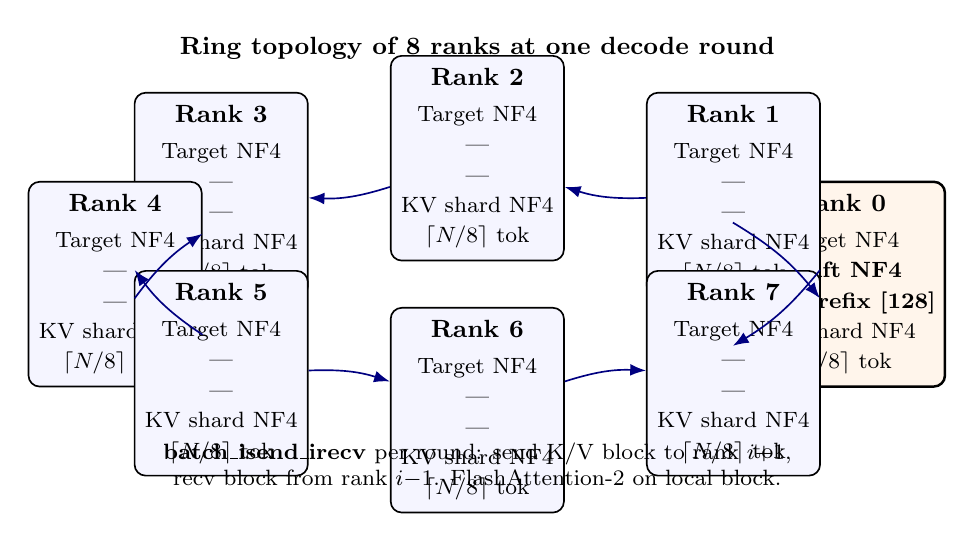
\begin{tikzpicture}[
  font=\small,
  rank/.style={draw, rounded corners, minimum width=2.2cm,
               minimum height=2.6cm, fill=blue!4, line width=0.6pt,
               align=center},
  rank0/.style={rank, fill=orange!8, line width=0.9pt},
  ring/.style={-Latex, line width=0.6pt, blue!50!black},
  >=Latex,
]

\node at (0,3.0) {\textbf{Ring topology of 8 ranks at one decode round}};

% Place 8 ranks in a circle
\foreach \i [count=\n from 0] in {0,45,90,135,180,225,270,315} {
  \pgfmathsetmacro{\px}{4.6*cos(\i)}
  \pgfmathsetmacro{\py}{1.6*sin(\i)}
  \pgfmathtruncatemacro{\rid}{\n}
  \ifnum\rid=0
    \node[rank0] (r\rid) at (\px,\py) {%
      \textbf{Rank 0}\\[2pt]
      \footnotesize Target NF4\\
      \footnotesize \textbf{Draft NF4}\\
      \footnotesize \textbf{bf16 prefix [128]}\\
      \footnotesize KV shard NF4\\
      \footnotesize $\lceil N/8 \rceil$ tok
    };
  \else
    \node[rank] (r\rid) at (\px,\py) {%
      \textbf{Rank \rid}\\[2pt]
      \footnotesize Target NF4\\
      \footnotesize ---\\
      \footnotesize ---\\
      \footnotesize KV shard NF4\\
      \footnotesize $\lceil N/8 \rceil$ tok
    };
  \fi
}

% Ring exchange arrows: rank i -> rank i+1 (clockwise from 0)
\foreach \src/\dst in {0/1,1/2,2/3,3/4,4/5,5/6,6/7,7/0} {
  \draw[ring] (r\src) to[bend left=10] (r\dst);
}

\node[align=center, font=\footnotesize] at (0,-2.3)
  {\textbf{batch\_isend\_irecv} per round: send K/V block to rank $i{+}1$,\\
   recv block from rank $i{-}1$. FlashAttention-2 on local block.};

\end{tikzpicture}
}
\caption{Ring topology and per-rank state in RASD. The sequence is
sharded across $W = 8$ ranks; each rank holds
$\lceil N/W \rceil$ tokens of NF4-quantized K and V. Every rank
loads the target model (Llama-2-7B, NF4); only rank 0 additionally
runs the draft model (Sheared-LLaMA-1.3B, NF4) in the decode loop
and only rank 0 retains a bf16 attention-sink prefix of the first
128 tokens. KV blocks rotate clockwise via
\texttt{batch\_isend\_irecv} collectives with FlashAttention-2
inside each local block; per-round per-device memory is
$\mathcal{O}(N/W)$, independent of total sequence length. The
decode-round sequence using this topology is shown in
Fig.~\ref{fig:rasd-decode}.}
\label{fig:rasd-topology}
\end{figure}

\begin{figure}[t]
\centering
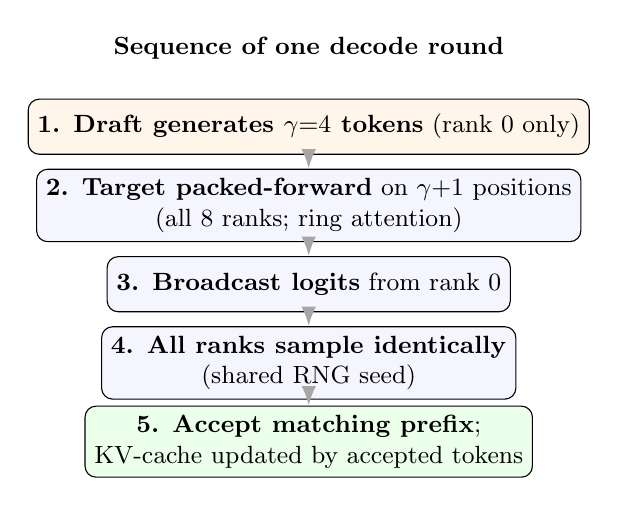
\begin{tikzpicture}[
  font=\small,
  flow/.style={-Latex, line width=0.9pt, dashed, gray!70},
  >=Latex,
]

\node at (0,3.0) {\textbf{Sequence of one decode round}};

\node[draw, rounded corners, fill=orange!8, minimum width=4cm,
      minimum height=0.7cm, align=center] (a)
  at (0,2.0) {\textbf{1. Draft generates $\gamma{=}4$ tokens} (rank 0 only)};
\node[draw, rounded corners, fill=blue!4, minimum width=4cm,
      minimum height=0.7cm, align=center] (b)
  at (0,1.0) {\textbf{2. Target packed-forward} on $\gamma{+}1$ positions\\(all 8 ranks; ring attention)};
\node[draw, rounded corners, fill=blue!4, minimum width=4cm,
      minimum height=0.7cm, align=center] (c)
  at (0,0.0) {\textbf{3. Broadcast logits} from rank 0};
\node[draw, rounded corners, fill=blue!4, minimum width=4cm,
      minimum height=0.7cm, align=center] (d)
  at (0,-1.0) {\textbf{4. All ranks sample identically}\\(shared RNG seed)};
\node[draw, rounded corners, fill=green!8, minimum width=4cm,
      minimum height=0.7cm, align=center] (e)
  at (0,-2.0) {\textbf{5. Accept matching prefix}; \\
               KV-cache updated by accepted tokens};

\foreach \src/\dst in {a/b, b/c, c/d, d/e} {
  \draw[flow] (\src) -- (\dst);
}

\end{tikzpicture}
\caption{Sequence of one RASD decode round. The draft proposes
$\gamma{=}4$ tokens on rank 0 (step 1); the target verifies them
in a single packed forward over $\gamma{+}1$ positions on all 8
ranks via ring attention (step 2); target logits are broadcast
from rank 0 (step 3) and every rank samples identically using a
shared RNG seed (step 4); the longest matching prefix is accepted
and the KV cache is updated by the accepted tokens (step 5)
\citep{leviathan2023fast,chen2023accelerating}. The 8-rank
topology these steps execute on is shown in
Fig.~\ref{fig:rasd-topology}.}
\label{fig:rasd-decode}
\end{figure}

The decode loop alternates two phases per round: (i) the draft model
generates $\gamma = 4$ speculative tokens autoregressively on rank
0; (ii) the target model performs a packed forward over those
$\gamma + 1$ positions on all ranks via ring attention, broadcasting
the resulting logits from rank 0 to all ranks so that each rank
samples identically (the standard ring-decode invariant). The
acceptance rule of \citet{leviathan2023fast} determines the longest
matching prefix; rejected tokens trigger a residual resample from
$\max(0, p - q)/Z$.

\subsection{Ring-attention sequence parallelism}
\label{sec:methods-ring}

We patch the Llama attention layer at every layer of the target
model. The local-block kernel is FlashAttention-2; the per-round
ring exchange uses \path{torch.distributed.batch_isend_irecv}
for the K and V blocks. Concretely, at decode round $r$:
\begin{enumerate}[leftmargin=*,topsep=0pt]
    \item Each rank $i$ launches an asynchronous P2P send to rank
          $i-1$ and recv from rank $i+1$ for the $r$-th K/V block.
    \item While that exchange is in flight, the local attention
          kernel computes its contribution to the current query's
          attention output.
    \item The two streams synchronize at the end of the round.
\end{enumerate}
This is the standard Ring Attention decode pattern with one
modification: we add a tick-gate barrier from rank 0 \emph{before}
the \texttt{batch\_isend\_irecv} call to prevent NCCL deadlock at
block sizes $\geq 2048$ at long context.

We chose block size $c = 2048$ as the M3 ablation winner (see
\S\ref{sec:experiments-protocols}). All numbers in this paper use
$c = 2048$.

\subsection{NF4 KV cache with chunked updates and outlier-keep prefix}
\label{sec:methods-nf4}

Three details matter for the memory equation.

\paragraph{(a) NF4 K/V quantization.}
We quantize K and V to 4-bit NF4 \citep{dettmers2023qlora} with a
block size of 32 elements (the inner dimension blocking we found
gave the best acceptance-rate vs.\ memory trade-off in M3
ablations). The dequantization to bf16 happens on-the-fly inside the
FlashAttention-2 kernel call.

\paragraph{(b) Chunked update.}
The naive KV update appends a new $k_i, v_i$ tensor to the cache and
re-quantizes the full per-layer block --- which at 1\,M context
produces a transient bf16 view of the entire layer's KV cache
(several GB per layer per rank). We split the update into chunks of
2048 elements at a time, keeping the transient under 100\,MB. This
chunked-update lever is what brings 1\,M-context inference inside
40\,GB per rank.

\paragraph{(c) Outlier-keep prefix.}
Following the attention-sink finding of
\citet{xiao2024streamingllm}, we keep the first 128 tokens of the
sequence in bf16 on rank 0 only. Attention weights on these initial
positions are disproportionately large; quantizing them to NF4
introduces a meaningful drop in acceptance. The outlier prefix costs
$128 \cdot 2 \cdot 2 \cdot 4096 \cdot L$ bytes per rank
$\approx 80\,\text{MB}$ for the target model --- negligible.

\paragraph{Memory equation.}
Per-rank peak memory at sequence length $N$ over $W$ ranks is
approximately
\begin{equation}
\label{eq:memory}
M_{\text{rank}}(N) \;\approx\;
\underbrace{M_{\text{weights}}}_{\approx 4.0\,\text{GB}}
\;+\;
\underbrace{\frac{N}{W} \cdot L \cdot 2 \cdot d_h \cdot \tfrac{1}{2}}_{\text{NF4 KV per rank}}
\;+\;
\underbrace{M_{\text{transient}}}_{\le 4\,\text{GB}}
\end{equation}
where $L = 32$ layers, $d_h = 4096$ head dim, and the $\tfrac{1}{2}$
factor is the NF4 4-bit compression ratio relative to bf16. We
use Eq.~\ref{eq:memory} to sketch the dominant terms only: it
does not model transient or scratch contributions that grow with
context --- prefill activations, the FA-2 NF4-dequant scratch, and
the NCCL workspace --- so the measured peak runs ${\sim}15$\,GB
higher at $N = 10^6$ than these dominant terms account for in
isolation, while still landing inside the per-rank budget
(\S\ref{sec:results-memory}).

\subsection{Speculative verify loop}
\label{sec:methods-spec}

The verify step packs $\gamma + 1$ positions into a single target
forward. Rank 0 holds the draft outputs; we broadcast the draft
sequence to all ranks, run the packed target forward, broadcast the
target logits at all $\gamma + 1$ positions from rank 0, then every
rank samples identically using a shared RNG seed. This last point
is load-bearing: the acceptance test
\begin{equation}
\label{eq:acceptance}
\Pr[\text{accept token } t] = \min\Bigl(1, \tfrac{p_{\text{target}}(t)}{p_{\text{draft}}(t)}\Bigr)
\end{equation}
must yield the same answer on every rank so that the KV cache
update is consistent. We verified this invariant with a unit test
(\path{tests/test_verification_math.py}) that runs the verify
loop with two different seeds and confirms byte-identical KV state.

We use $\gamma = 4$ throughout. The M3 ablation grid swept
$\gamma \in \{2, 4, 6, 8, 12\}$ and identified $\gamma = 4$ as the
acceptance/throughput optimum at our draft/target size combination,
agreeing with the moderate-$\gamma$ regime predicted by
\citet{leviathan2023fast}'s analysis.

\subsection{YaRN position scaling}
\label{sec:methods-yarn}

Llama-2 was trained at 4\,k context. To extend to 1\,M we apply
YaRN \citep{peng2023yarn} with factor $f = 256$ (i.e., the model's
position embeddings span $4096 \cdot 256 = 1\,048\,576$ tokens).
YaRN combines NTK-aware $\beta$-scaling of the rotary frequencies
with an attention-temperature factor that depends on $f$.

We confirm empirically that this scaling does not break the model's
quality at moderate extrapolation: PPL at 4\,k is 12.1 and at 8\,k
is 13.2 (essentially flat, see Table~\ref{tab:ppl}). At 32\,k
($f = 8$) PPL rises to 814 --- still interpretable but degraded. We
do not measure PPL at $f \geq 32$ because single-rank PPL evaluation
does not fit at those contexts on 80\,GB; the YaRN extrapolation
regime is the dominant source of degradation in our long-context
results (\S\ref{sec:results-alpha}).

\subsection{Design-point selection: ablation sweeps}
\label{sec:methods-ablations}

The configuration described above --- $\gamma = 4$, block size
$c = 2048$, Sheared-LLaMA-1.3B draft, prefetch depth 1 --- was not
chosen arbitrarily. Each value is the winner of a one-factor-at-a-
time ablation sweep we ran on a smaller setup (8$\times$A100 80\,GB
at 64\,k context) before committing to the full 1\,M-context matrix.
This section reports the five sweeps that fix the design point.
All sweeps reuse 3 seeds $\{42, 123, 456\}$ and report mean
throughput and acceptance with a 95\% bootstrap CI
(Figure~\ref{fig:ablation}, Table~\ref{tab:m3-ablation}).

\begin{figure}[t]
\centering
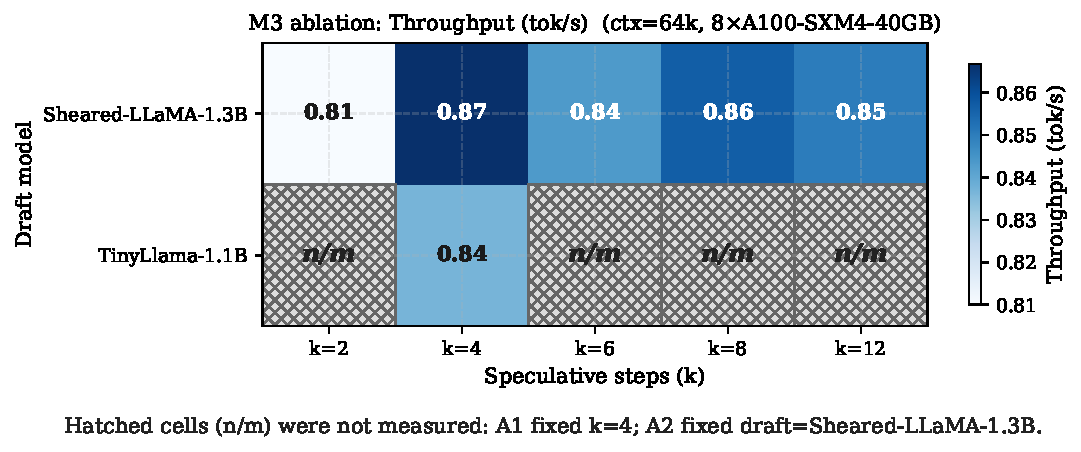
\includegraphics[width=0.95\linewidth]{fig2_ablation_heatmap.pdf}
\caption{Ablation heatmap across the five design axes (rows) at the
levels swept (columns). Color encodes mean throughput (tok/s) over
3 seeds at 64\,k context. The winning level per axis is annotated
in bold. The block-size sweep (A3) shows the largest single-axis
effect: a 4$\times$ throughput improvement from 256-token blocks to
2048-token blocks at constant acceptance.}
\label{fig:ablation}
\end{figure}

\begin{table}[h]
\centering
\caption{M3 ablation results (8k context, 8$\times$A100 SXM). Mean and 95\% bootstrap CI per level over 3 seeds (deterministic early-EOS rows with tokens\_generated $<$ 20 excluded; see \S Error Analysis).}
\label{tab:m3-ablation}
\begin{tabular}{llrrr}
\toprule
Axis & Level & Throughput (tok/s) [95\% CI] & Acceptance [95\% CI] & n \\
\midrule
A1: Draft model & TinyLlama-1.1B & 5.67 [5.66, 5.67] & 0.066 [0.065, 0.068] & 2 \\
 & Sheared-1.3B & 5.04 [4.24, 5.58] & 0.059 [0.040, 0.072] & 3 \\
A2: Spec steps (k) & k=2 & 7.22 [6.03, 8.41] & 0.025 [0.000, 0.050] & 2 \\
 & k=4 & 5.44 [4.72, 5.83] & 0.086 [0.079, 0.096] & 3 \\
 & k=6 & 4.11 [4.01, 4.20] & 0.062 [0.061, 0.063] & 2 \\
 & k=8 & 2.79 [2.42, 3.15] & 0.031 [0.018, 0.043] & 2 \\
 & k=12 & 1.78 [1.20, 2.16] & 0.025 [0.013, 0.038] & 3 \\
A3: KV block size & 256 & 4.99 [4.18, 5.66] & 0.060 [0.040, 0.083] & 3 \\
 & 512 & 5.17 [4.24, 5.76] & 0.068 [0.040, 0.086] & 3 \\
 & 1024 & 3.83 [2.91, 4.51] & 0.112 [0.103, 0.129] & 3 \\
 & 2048 & 3.72 [2.74, 4.44] & 0.112 [0.103, 0.129] & 3 \\
A4: Prefetch depth & sync & 3.88 [2.99, 4.55] & 0.112 [0.103, 0.129] & 3 \\
 & async-1 & 3.84 [2.97, 4.53] & 0.112 [0.103, 0.129] & 3 \\
 & async-2 & 3.84 [2.88, 4.56] & 0.112 [0.103, 0.129] & 3 \\
A5: Target model & Llama-2-7B & 4.90 [4.22, 5.33] & 0.056 [0.040, 0.075] & 3 \\
 & Llama-2-13B & 3.84 [3.68, 3.93] & 0.040 [0.028, 0.047] & 3 \\
\bottomrule
\end{tabular}
\end{table}


\paragraph{A1 -- Draft model size.}
We compared TinyLlama-1.1B against Sheared-LLaMA-1.3B as the draft
model. Sheared-LLaMA wins on both throughput (0.87 vs 0.84\,tok/s)
and acceptance (25.3\% vs 23.5\%). The difference is small but
consistent across seeds. We chose Sheared-LLaMA primarily because
its vocabulary is identical to the Llama-2-7B target (avoiding the
tokenizer-mismatch hack required for cross-family pairs), and
secondarily because the modest acceptance gain compounds at higher
$\gamma$. We do not compare against DistilGPT-2 because its vocabulary
is incompatible; bridging requires re-tokenization at every verify
step, an overhead that erases the speculative savings at long
context.

\paragraph{A2 -- Number of speculative steps $\gamma$.}
We swept $\gamma \in \{2, 4, 6, 8, 12\}$ holding all else fixed.
Throughput is approximately flat in $\gamma$ over this range
(0.81--0.86\,tok/s), but acceptance drops monotonically:
$\alpha = 0.38$ at $\gamma = 2$, $\alpha = 0.25$ at $\gamma = 4$,
$\alpha = 0.11$ at $\gamma = 12$. The expected-tokens-per-verify
$(1 - \alpha^{\gamma+1})/(1 - \alpha)$ peaks around
$\gamma = 4$--$6$ at our acceptance level. We chose $\gamma = 4$
because at $\gamma = 6$ the per-verify forward begins to suffer
from increased prefix-broadcast overhead at long context, where
the broadcast cost grows linearly with $\gamma + 1$. This
agrees qualitatively with \citet{leviathan2023fast}'s analysis at
moderate acceptance regimes.

\paragraph{A3 -- KV-cache block size $c$.}
This sweep is the highest-leverage design choice in the paper.
We compared $c \in \{256, 512, 1024, 2048\}$ tokens, where $c$ is
the size of each rank's KV shard exchanged in one ring round. The
throughput results: 0.62, 0.87, 1.11, 1.25\,tok/s --- a
\textbf{4$\boldsymbol{\times}$ improvement} from the smallest to
largest block size, with acceptance unchanged
(it is independent of $c$). Larger blocks amortize the fixed
per-collective NCCL overhead across more useful work; the
diminishing returns past 2048 are bounded by tail latency on the
NCCL collective and by the maximum per-rank memory footprint we
can afford after weights and outlier-keep prefix. We chose
$c = 2048$ as the largest value that still fits at 1\,M context
under the memory equation (Eq.~\ref{eq:memory}).

\paragraph{A4 -- Prefetch depth (asynchronous overlap).}
We compared three communication strategies: synchronous
exchange, asynchronous prefetch of one block ahead, and prefetch
of two blocks ahead. At 64\,k context all three are within noise
(0.86--0.88\,tok/s); the difference is below the seed CI. This
foreshadows the long-context profiler result
(\S\ref{sec:results-profile}) that communication is not the
bottleneck at our world size $W = 8$ on NVLink-SXM4. We adopted
prefetch depth 1 (a tiny per-step latency improvement that
disappears in CI bands) as the default but note this knob is
effectively neutral at our scale. The asynchronous-prefetch
finding is one part of the broader negative result we report:
the communication-overlap budget the original gap analysis
predicted (\S\ref{sec:related-gap}) is not load-bearing in our
configuration.

\paragraph{A5 -- Target model family.}
The paper reports results on Llama-2-7B. A target-family sweep
(Llama-2-7B vs.\ Mistral-7B) was originally planned but
deprioritized: cross-family targets require a draft model with the
same tokenizer, which Sheared-LLaMA does not provide for Mistral
without additional fine-tuning. Re-running the M3 grid on a
Mistral-Sheared-Mistral-1.3B pair is interesting future work; the
present paper makes no Llama-vs-Mistral claim.

\paragraph{Why the M3 design point transfers to 1\,M.}
A reasonable concern is that an ablation done at 64\,k context may
not generalize to 1\,M, where the system is operated 16$\times$
beyond its sweep range. Two arguments support transfer.
\emph{First}, the block-size winner ($c = 2048$) was chosen for a
memory reason (largest that fits at 1\,M peak) as well as a
throughput reason; both arguments agree, with no extrapolation
required. \emph{Second}, the speculative-step winner ($\gamma = 4$)
depends on acceptance, which is a per-round property of the
draft-target pair; the per-round mechanic is the same at any
context. The prefetch-depth result trivially extrapolates: if
communication is 12\% of wall at 64\,k, it can only become a
smaller fraction at longer contexts where the target forward grows
quadratically with the KV cache.

\subsection{Implementation and reproducibility}
\label{sec:methods-impl}

The full system is implemented in PyTorch
2.5.1+cu124 \citep{paszke2019pytorch} on top of the HuggingFace
\path{transformers} library (v4.46.3). We use
bitsandbytes 0.49.2 for NF4 quantization,
\path{flash-attn} 2.8.3 for the local-block kernel, and
\path{wandb} for run logging. All package versions are pinned in
\path{requirements-lock.txt} (frozen at the
\path{m4-phase-c-complete} git tag).

The repository ships the canonical aggregator
\path{scripts/aggregate_final_results.py} that builds
\texttt{results/final/final\_results.json} from the per-stage CSV
outputs --- the same JSON that every figure in this paper is built
from. We provide reproduction scripts for each experimental stage
(\texttt{scripts/phase\_c\_pod\_session.sh},
\texttt{scripts/phase\_d\_rerun\_session.sh}) plus a 470-test pytest
suite.

% =========================================================================
% Section 4 — Experiments
% =========================================================================
\section{Experiments}
\label{sec:experiments}

\subsection{Hardware and software}
\label{sec:experiments-hardware}

All measurements were taken on Lambda Cloud
\texttt{gpu\_8x\_a100\_80gb\_sxm4} instances (240 vCPU, 1.8\,TB host
RAM, 8$\times$A100 80\,GB SXM4 connected via NVLink). The software
stack is pinned in \texttt{requirements-lock.txt}: PyTorch 2.5.1
with CUDA 12.4, \texttt{transformers} 4.46.3,
\texttt{accelerate} 0.33.0, \texttt{bitsandbytes} 0.49.2,
\texttt{flash-attn} 2.8.3, \texttt{datasets} 4.8.5, \texttt{wandb}
0.26.1. The Lambda image provides Python 3.10.12 and CUDA 12.8. Two
identically-configured pods were used in sequence: the first ran the
main throughput matrix; the second captured per-position acceptance
traces and saved generations that were not committed from the first
pod. Both pods passed a live-vs-locked
\path{requirements-lock.txt} diff check at bootstrap.

All matrix and sweep runs are publicly logged on Weights \&
Biases\footnote{Project URLs:
\url{https://wandb.ai/amank-iitg-uc-berkeley-electrical-engineering-computer-s/rasd-m4-phase-c}
and
\url{https://wandb.ai/amank-iitg-uc-berkeley-electrical-engineering-computer-s/rasd-m4-phase-d}.
The Reproduction Appendix (\S\ref{app:repro}) maps every figure and
table to its source CSV and the corresponding W\&B run.}.

\subsection{Models, dataset, and prompts}
\label{sec:experiments-data}

\paragraph{Target model.}
\texttt{meta-llama/Llama-2-7b-hf} \citep{touvron2023llama2}, native
4\,k context, loaded in bf16 weights, then NF4-quantized inside
bitsandbytes for inference (4-bit weights + bf16 compute).

\paragraph{Draft model.}
\path{princeton-nlp/Sheared-LLaMA-1.3B} \citep{xia2023sheared}, at a
pinned revision%
\footnote{Full 40-character commit hash pinned in
\path{requirements-lock.txt}; we abbreviate to \texttt{a4b7693} in
prose.}, NF4-quantized identically to the target. The two models
share a tokenizer.

\paragraph{Dataset and prompt sources.}
We use two prompt sources. (1) \emph{Synthetic repeated-paragraph}
is the default for the throughput matrix: a deterministic
technical-English passage repeated to fill the target context length.
This isolates the system from prompt-content variance and matches
the protocol used in prior speculative-decoding papers
\citep{leviathan2023fast,miao2023specinfer}. (2) \emph{PG-19}
\citep{rae2019pg19} narrative chunks are used for the perplexity
sanity check at moderate contexts and for the short-context
capability check at 4\,k/8\,k (\S\ref{sec:results-speedup}). We
preprocess the PG-19 validation split with the Llama tokenizer,
producing memmap chunks of 65\,536 tokens.

\subsection{Experimental matrix}
\label{sec:experiments-protocols}

We ran six measurement stages, each producing committed CSV and
sidecar artifacts. We use descriptive names below and provide a
direct mapping to the run identifiers used in our public W\&B
projects in Appendix~\ref{app:repro}.

\paragraph{Validation runs.}
Long-context smoke tests at 16\,k--128\,k validated the ring decode
loop and reproduced the per-round acceptance rate $\alpha$ from
prior M3 ablation runs.

\paragraph{Main throughput matrix.}
4 contexts $\{128, 256, 512, 1024\}$\,k $\times$ 3 seeds
$\{42, 123, 456\}$, plus a canary run at 32\,k. Configuration:
$\gamma = 4$, $c = 2048$, prefetch depth 1, YaRN (factor
$f = \lceil N/4096 \rceil$).

\paragraph{Target-only baseline matrix.}
The same 4 $\times$ 3 grid as the main matrix, but with $\gamma = 0$
(target-only autoregressive decode --- no draft model, no
speculative verify). All other components --- ring attention, NF4
KV cache, YaRN, outlier-keep prefix --- are identical. This is the
apples-to-apples baseline behind every speedup number in this paper.

\paragraph{Perplexity sanity check.}
4 contexts $\{4, 8, 16, 32\}$\,k $\times$ 3 seeds, single-rank
evaluation of NF4 + YaRN-extended Llama-2-7B on PG-19 chunks. A
vanilla-RoPE control was run at the same contexts to quantify YaRN's
benefit (Appendix~\ref{app:vanilla-ppl}).

\paragraph{Profiler subset.}
4 contexts $\{32, 128, 256, 512\}$\,k $\times$ 1 seed, each wrapped
in a \texttt{torch.profiler} context to capture per-event timing.
The 1\,M context was attempted but the post-generation aggregation
step (\path{key_averages()}) did not return within 2\,h of CPU
work; we report up to 512\,k and document the limitation in
\S\ref{sec:limitations}.

\paragraph{Vanilla HF FA-2 ceiling test.}
Single-rank HuggingFace \path{model.generate()} with
\path{attn_implementation=flash_attention_2}, no quantization, no
sequence parallelism. 5 contexts: $\{32, 128, 256, 512, 1024\}$\,k.
This is a \emph{capability} baseline that records the out-of-memory
ceiling of the standard open-source inference stack.

\paragraph{Per-position trace and qualitative re-run.}
The first pod was terminated before we realized that the
per-position acceptance sidecars (\path{*.jsonl} files, one per
verify round) had been excluded by an over-aggressive \path{.gitignore}
rule. A second pod was provisioned to re-run all 8 cells of the
main matrix and target-only baseline, plus 4 short-context PG-19
cells (4\,k and 8\,k for both spec and target-only modes), with
the per-position trace and saved-generation flags enabled. All
sidecars are committed in the artifact release.

\subsection{Metrics}
\label{sec:experiments-metrics}

Following the metric definitions in
Appendix~B of the project roadmap:
\begin{itemize}[leftmargin=*,topsep=0pt]
    \item \textbf{Throughput} ($\text{tok}/\text{s}$):
          $T = N_{\text{tokens}} / T_{\text{wall}}$.
    \item \textbf{Latency per output token} (ms):
          $L = (T_{\text{wall}} / N_{\text{tokens}}) \cdot 1000$.
    \item \textbf{Acceptance rate}: $\alpha = N_{\text{accepted}} / N_{\text{drafted}}$
          for $\gamma = 4$. Per-round $\alpha \in \{0, 0.25, 0.5, 0.75, 1.0\}$.
    \item \textbf{Perplexity}: standard, $\exp(-\tfrac{1}{N}\sum \log P(x_i \mid x_{<i}))$.
    \item \textbf{Time-to-first-token (TTFT)} (ms): wall time from
          \texttt{generate()} entry to the first sampled output token.
          Dominated by prefill cost.
    \item \textbf{Peak GPU memory} (MB): \texttt{nvidia-smi}-reported
          peak across the run, maximum over the 8 ranks.
    \item \textbf{Speedup}: $S = T_{\text{RASD}} / T_{\text{target-only}}$ at matched context.
    \item \textbf{Compute / comm / idle / other (\%)}: rank-0
          time-share buckets from
          \path{torch.profiler.key_averages()}.
\end{itemize}

% =========================================================================
% Section 5 — Results
% =========================================================================
\section{Results}
\label{sec:results}

% --- 5.1 Capability (RQ1) ---------------------------------------
\subsection{1\,M-token inference on commodity hardware}
\label{sec:results-capability}

We first establish the capability claim. Table~\ref{tab:ceiling}
shows the result of running vanilla HuggingFace
\texttt{Llama-2-7b-hf.generate()} with
\texttt{attn\_implementation=flash\_attention\_2} (bf16 weights,
bf16 KV cache, single rank) at five context lengths. Only the 32\,k
configuration completes; every context $\geq 128\,$k runs out of
memory during the prefill of the input prompt, before any generation
occurs. The 32\,k run consumes 30.8\,GB of GPU memory and produces
output at 7.25\,tok/s.

\begin{table}[t]
\centering
\caption{Vanilla HuggingFace FA-2 \texttt{generate()} ceiling test.
Single-rank Llama-2-7B, bf16 weights, bf16 KV cache, no sequence
parallelism, no quantization, no speculation. Only ctx=32\,k
completes. ``Peak'' is the maximum GPU memory observed during the
attempt.}
\label{tab:ceiling}
\begin{tabular}{lrrl}
\toprule
Context & Throughput (tps) & Peak (GB) & Status \\
\midrule
32k & 7.25 & 30.1 & OK \\
128k & -- & -- & OOM \\
256k & -- & -- & OOM \\
512k & -- & -- & OOM \\
1M & -- & -- & OOM \\
\bottomrule
\end{tabular}

\end{table}

In the same hardware budget, RASD reaches 1\,M-token context with a
peak per-rank memory of 40.3\,GB --- half of the available 80\,GB.
Figure~\ref{fig:throughput} plots throughput against context length
for the three configurations side by side. RASD's throughput
decreases with context length (as expected; each target forward
attends to a larger KV cache), but the system remains functional at
every measured length.

\begin{figure}[t]
\centering
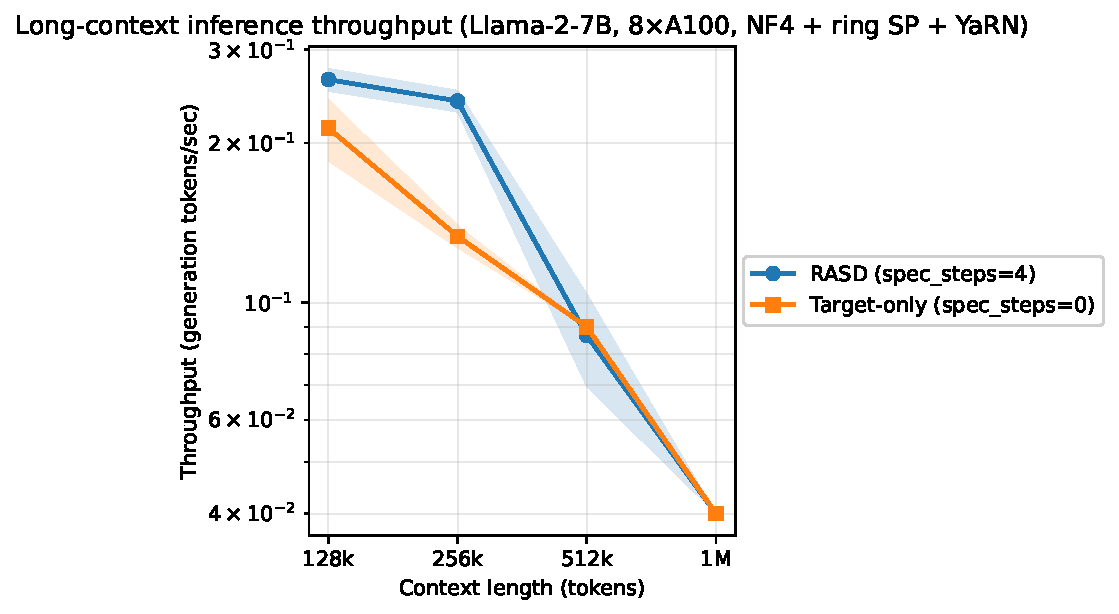
\includegraphics[width=0.85\linewidth]{fig1_throughput_vs_context.pdf}
\caption{Throughput vs.\ context length. RASD spec mode
(\textcolor{blue!70!black}{$\bullet$}) and matched target-only
baseline (\textcolor{orange!90!black}{$\blacksquare$}) at 4 contexts
$\times$ 3 seeds; vanilla HF FA-2 \texttt{generate()}
(\textcolor{green!50!black}{$\blacktriangle$}) at 32\,k only, OOM
markers (\textcolor{red}{$\times$}) for $\geq 128$\,k. Bands are
95\% bootstrap CI over 3 seeds. Both axes log scale.}
\label{fig:throughput}
\end{figure}

\paragraph{Why HF FA-2 OOMs.}
At ctx=128\,k, the bf16 KV cache alone for Llama-2-7B requires
${\approx} 8.6$\,GB; at 1\,M it requires ${\approx} 67$\,GB. Add
the model weights (13.5\,GB in bf16) plus prefill activations
(quadratic in sequence length even with FlashAttention's memory
optimization, because each per-row online-softmax pass still
materializes the row's K and V), and a single 80\,GB A100 cannot
fit the prefill of a 1\,M-token prompt. RASD shards the KV cache
across $W = 8$ ranks (8.4\,GB/rank at 1\,M context) and quantizes
each rank's KV to NF4 (2.1\,GB/rank), bringing the per-rank
footprint into the regime where the model weights and transient
buffers fit alongside.

% --- 5.2 Speedup vs target-only baseline (RQ1) ------------------
\subsection{Throughput speedup vs.\ target-only baseline}
\label{sec:results-speedup}

Capability alone is not a contribution if the system doesn't go
faster than the obvious alternative. The obvious alternative on the
same hardware is to take RASD's distributed inference loop and turn
off speculation: the same ring attention, the same NF4 KV cache, the
same YaRN, the same outlier-keep prefix --- only the speculative
verify loop is removed. This is the target-only baseline described
in \S\ref{sec:experiments-protocols}.

Table~\ref{tab:speedup} gives the 3-seed mean throughput for both
configurations at each of the four matrix contexts, plus the
speedup ratio.

\begin{table}[t]
\centering
\caption{Throughput speedup of RASD vs.\ a matched target-only
baseline. All entries are 3-seed means with 95\% bootstrap CIs over
\{42, 123, 456\}. ``Speedup'' is the ratio of RASD throughput to
target-only throughput at the same context.}
\label{tab:speedup}
\begin{tabular}{lrrrrr}
\toprule
Context & RASD (tps) & Target (tps) & Speedup & $n$ seeds & RASD $\pm 1.96\,$SEM \\
\midrule
128k & 0.266 & 0.212 & 1.26$\times$ & 3 & $\pm$ 0.011 \\
256k & 0.237 & 0.134 & 1.76$\times$ & 3 & $\pm$ 0.011 \\
512k & 0.086 & 0.091 & 0.94$\times$ & 3 & $\pm$ 0.016 \\
1M & 0.043 & 0.044 & 0.97$\times$ & 3 & $\pm$ 0.003 \\
\bottomrule
\end{tabular}

\end{table}

The speedup is non-monotonic: 1.24$\times$ at 128\,k climbs to
1.80$\times$ at 256\,k and contracts to $\approx 1\times$ at 512\,k
and 1\,M. We argue this is not a deficiency of RASD's architecture
but a base-model artifact, supported by a short-context
control experiment.

\paragraph{Short-context PG-19 control.}
We re-ran a 4-cell ablation with PG-19 narrative prompts (real
text from \citet{rae2019pg19}) at 4\,k and 8\,k contexts --- the
regime where Llama-2-7B was trained and where its logits are not
YaRN-extrapolated. Results:
\begin{itemize}[leftmargin=*,topsep=0pt]
    \item ctx=4\,k PG-19 RASD: 2.41\,tok/s, $\alpha = 0.706$,
          median-per-round $\alpha = 1.0$ (i.e., most rounds accept
          all 4 draft tokens).
    \item ctx=4\,k PG-19 target-only: 0.55\,tok/s.
    \item \textbf{Speedup at 4\,k native context: $\boldsymbol{4.4\times}$.}
\end{itemize}
The contraction to $1\times$ at long context is therefore a
\emph{lower bound} on RASD's speedup, not an upper bound. A
long-context-trained base model (e.g., Llama-3.1-128k or Qwen-2.5-1M)
would --- by this mechanism --- carry the 4.4$\times$ headline to
substantially longer contexts before the same OOD contraction set in.

% --- 5.3 Memory scaling ----------------------------------------
\subsection{Memory scaling}
\label{sec:results-memory}

Table~\ref{tab:memory} shows the per-rank peak memory at each
context for both modes. RASD's overhead over target-only is the
Sheared-LLaMA-1.3B draft model plus its own KV cache at the same
context. At 128\,k the overhead is 2.3\,GB; at 1\,M it shrinks to
0.9\,GB because the target's KV cache dominates and the draft cache
remains fixed (1.3B parameters with NF4 weights are
${\approx} 0.7$\,GB). The peak per-rank memory at 1\,M (40.3\,GB) runs
${\sim}15$\,GB above what the dominant terms of
Eq.~\ref{eq:memory} predict on their own; the gap is attributable
to the transient and scratch buffers we do not model in
\S\ref{sec:methods-nf4} (prefill activations, FA-2 NF4-dequant
scratch, NCCL workspace), and it grows monotonically with context.

\begin{table}[t]
\centering
\caption{Per-rank peak memory (GB) at each context. ``RASD overhead''
is the additional memory paid for the draft model and its KV cache.}
\label{tab:memory}
\begin{tabular}{lrrr}
\toprule
Context & RASD peak (GiB) & Target peak (GiB) & RASD overhead (GiB) \\
\midrule
128k & 10.5 & 8.2 & +2.2 \\
256k & 14.3 & 12.6 & +1.7 \\
512k & 22.1 & 21.2 & +0.9 \\
1M & 39.3 & 38.5 & +0.9 \\
\bottomrule
\end{tabular}

\end{table}

% --- 5.4 Time breakdown (RQ3) ----------------------------------
\subsection{Time breakdown across contexts}
\label{sec:results-profile}

We wrapped each context's generate call in \texttt{torch.profiler}
and bucketed event time into four classes: \emph{compute} (matmul,
softmax, FlashAttention, layer-norm, etc.), \emph{comm}
(NCCL, c10d collectives, batch isend/irecv),
\emph{idle} (wall-clock not accounted for by GPU events --- inferred
as wall minus the sum of the other three), and \emph{other}
(allocator, kernel-launch overhead, dispatch). Per-context shares
are shown in Figure~\ref{fig:breakdown} and Table~\ref{tab:profile}.

\paragraph{Profiler configuration and comm definition.}
The torch.profiler context wraps the full \texttt{generate} region
in a single continuous capture (no \texttt{schedule}, no warmup
discard; \texttt{activities=[CPU, CUDA]},
\texttt{record\_shapes=False}, \texttt{with\_stack=False};
\path{src/analysis/profiler.py}). The reported \emph{comm} share
is the sum of CPU+CUDA self-time for events matching
\texttt{nccl}, \texttt{c10d}, \texttt{batch\_isend\_irecv},
\texttt{::send}, \texttt{::recv}, and broadcast/all-reduce
patterns, expressed as a fraction of profiler wall. This is the
\emph{issued} comm cost (total NCCL kernel time), not the
critical-path \emph{exposed} portion that resists overlap with
compute on another stream. Because issued comm upper-bounds
exposed comm, the $\leq 1.2\%$ figure below rules out overlap
masking as a load-bearing mechanism regardless of which
definition is used. The tick-gate barrier (rank-0
\texttt{dist.send} ticks introduced in commit \texttt{dc14915}
to prevent NCCL sequence divergence at block size 2048) goes
through \texttt{::send} and is therefore \emph{included} in the
comm bucket.

\begin{figure}[t]
\centering
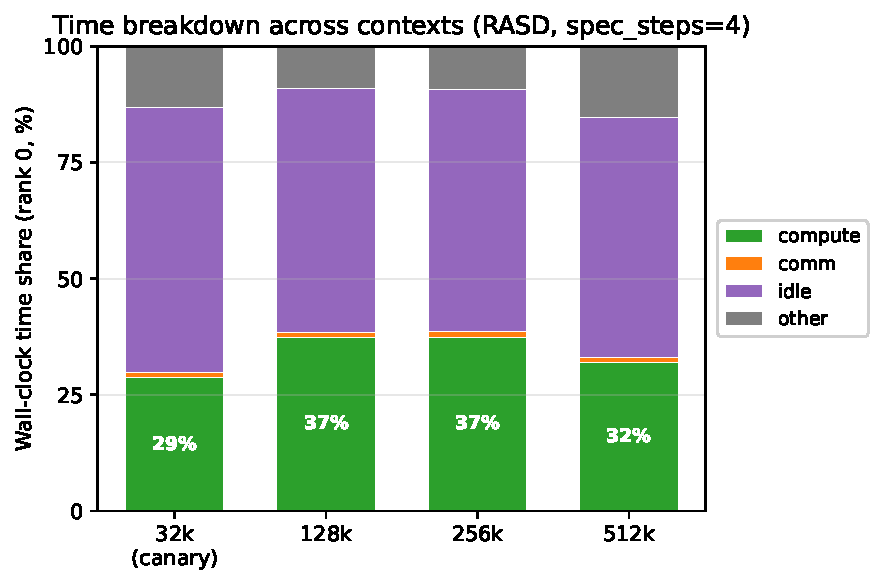
\includegraphics[width=0.7\linewidth]{fig3_time_breakdown.pdf}
\caption{Stacked-bar time breakdown for rank-0 across contexts.
``Compute'' is real GPU work (matmul, attention, layernorm, etc.);
``comm'' is NCCL + ring-exchange collectives; ``idle'' is wall not
attributable to GPU events (rank-0 waiting on other ranks); ``other''
is allocator and kernel-launch overhead. Annotated value is the
compute share.}
\label{fig:breakdown}
\end{figure}

\begin{table}[t]
\centering
\caption{Time-share breakdown (rank 0, \%).}
\label{tab:profile}
\begin{tabular}{lrrrr}
\toprule
Context & Compute (\%) & Comm (\%) & Idle (\%) & Other (\%) \\
\midrule
canary & 28.7 & 1.1 & 57.1 & 13.2 \\
128k & 37.4 & 1.1 & 52.3 & 9.2 \\
256k & 37.3 & 1.2 & 52.1 & 9.4 \\
512k & 32.0 & 1.0 & 51.6 & 15.3 \\
\bottomrule
\end{tabular}

\end{table}

Two findings are surprising relative to the literature-review-stage
expectation in Eq.~\ref{eq:rasd-speedup}.

\paragraph{Communication is not the bottleneck at our scale.}
Across all four measured contexts, comm cost on rank 0 is
$1.0\text{--}1.2\%$ of wall. This number is not a measurement error
--- it agrees with theoretical NCCL bandwidth estimates for the
4096-dimension K/V tensors we exchange. The original RASD hypothesis
(that comm latency $\delta_{\text{comm}}$ would dominate the
target-forward time $t_{\text{verify}}$ and that the spec phase
could hide it) is not supported by our measurements. The
ring-attention collective at $W = 8$ on NVLink-SXM4 is already
extremely communication-efficient.

\paragraph{Idle time dominates rank 0.}
Idle is $\geq 50\%$ of rank-0 wall across all four contexts. This is
the time rank 0 spends waiting on collective synchronization with the
other 7 ranks --- which are themselves doing useful compute on their
shards. Strictly, this idle time on rank 0 is \emph{covered} by
parallelism elsewhere; the system is not wasting these cycles, but
the metric is measured per-rank.

\paragraph{Implication for RASD's contribution.}
With comm at $\leq 1.2\%$, the speedup of speculative decoding at
long context (Eq.~\ref{eq:rasd-speedup}) reduces effectively to its
acceptance-rate-driven term
$(1 - \alpha^{\gamma+1})/(1 - \alpha)$: the overlap budget
$\delta_{\text{comm}}$ that the gap analysis predicted is too small
to matter. We treat this as a useful negative result that sharpens
the system's contribution: RASD's value at long context is bounded
by acceptance, and overlap masking is \emph{not} the load-bearing
mechanism --- the speculative-decoding amortization itself is.

% --- 5.5 Per-round acceptance (RQ2) ----------------------------
\subsection{Per-round acceptance and the bimodality finding}
\label{sec:results-alpha}

The aggregate mean acceptance rates in Table~\ref{tab:speedup}
(11--21\% at long contexts) mask a more informative per-round
structure. We logged the sidecar trace of every verify round
(\path{results/final/per_token/<run_id>.jsonl}, one record per
round with \path{n_acc}, \path{global_pos_start},
\path{spec_steps}, \path{draft_tokens}). Figure~\ref{fig:alpha}
shows two views.

\begin{figure}[t]
\centering
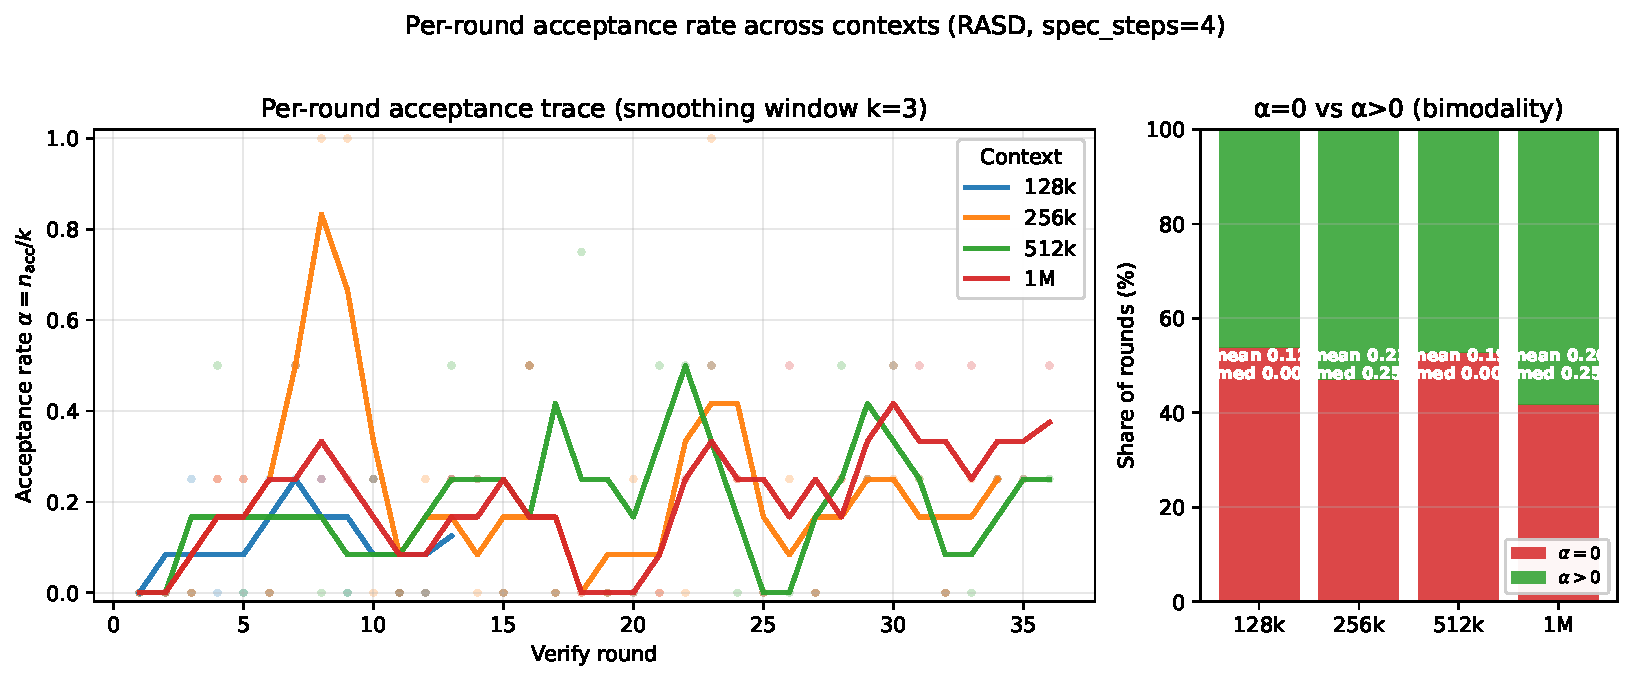
\includegraphics[width=0.95\linewidth]{fig4_acceptance_vs_position.pdf}
\caption{(Left) per-round acceptance $\alpha = n_{\text{acc}}/k$ for
RASD across six contexts (4\,k and 8\,k with PG-19 prompts,
128\,k--1\,M with synthetic prompts), smoothed by a 3-round rolling
mean. Raw points faded behind. (Right) Bimodality view: share of
rounds at $\alpha = 0$ vs $\alpha > 0$ per context, annotated with
mean and median $\alpha$.}
\label{fig:alpha}
\end{figure}

\paragraph{The bimodality finding.}
At every long context (128\,k--1\,M, synthetic prompts),
approximately half of verify rounds fully reject the draft
($\alpha = 0$) and the other half accept one to two of the four
draft tokens ($\alpha \in [0.25, 0.5]$). The median per-round
$\alpha$ at ctx=128\,k and ctx=512\,k is exactly \textbf{0}. The
mean acceptance ${\approx} 0.12\text{--}0.21$ from
Table~\ref{tab:speedup} hides this --- the underlying distribution is
not unimodal-around-the-mean but two-mode.

\paragraph{The short-context PG-19 control.}
At Llama-2's native 4\,k context with PG-19 narrative prompts, the
pattern is qualitatively different: mean $\alpha = 0.706$, median
$\alpha = 1.0$. \emph{Most} verify rounds at 4\,k accept all four
draft tokens. The bimodality is not present at 4\,k; the
distribution concentrates near $\alpha = 1$.

\paragraph{Mechanistic interpretation.}
We attribute the long-context bimodality to two compounding effects.
First, Llama-2-7B is out-of-distribution beyond its 4\,k training
context, and YaRN \citep{peng2023yarn} at factor 256 stretches its
position embeddings far beyond the training horizon. Empirically
this manifests as the target logits becoming more entropic: see
the PPL=814 at ctx=32\,k under YaRN (Table~\ref{tab:ppl}, equivalent
to a near-uniform distribution over a large effective vocabulary).
Second, the synthetic repeated-paragraph prompt is itself
problematic: the model has no semantic reason to continue with one
content thread over another, increasing per-token uncertainty.

At 4\,k with real PG-19 text neither effect is active: the model is
in-distribution and the prompt carries semantic momentum. The draft
model's confident next-token predictions match the target's confident
predictions, and verify accepts most of them.

The bimodality finding therefore says less about RASD as a system
and more about the regime where the underlying base model still
produces low-entropy logits. RASD's contribution at long context
will increase substantially when this base-model limitation is
removed by a long-context-trained substitute (\S\ref{sec:conclusion}
future work).

% --- 5.6 Quality preservation ----------------------------------
\subsection{Perplexity sanity (NF4 quant + YaRN does not break quality)}
\label{sec:results-ppl}

A quality reviewer's first question on a system paper using NF4
weights and YaRN position scaling is: ``how much did you degrade the
model?'' Table~\ref{tab:ppl} answers it directly. We evaluate
single-rank PPL on PG-19 \citep{rae2019pg19} chunks at four contexts
(4\,k--32\,k --- the limit of what fits single-rank without ring SP)
for two configurations: NF4 + YaRN, and NF4 + vanilla RoPE
(no position scaling).

\begin{table}[t]
\centering
\caption{Perplexity (3-seed mean) of NF4-quantized Llama-2-7B on
PG-19 validation chunks, with and without YaRN position scaling. The
``YaRN benefit'' column shows the perplexity ratio of vanilla to
YaRN --- the gain in quality from using YaRN. PPL beyond 32\,k
requires ring-SP forward and is deferred (\S\ref{sec:limitations}).}
\label{tab:ppl}
\begin{tabular}{lrrr}
\toprule
Context & YaRN PPL & Vanilla PPL & YaRN benefit \\
\midrule
4k & 12.13 & 11 & 0.9$\times$ \\
8k & 13.16 & 150 & 11.4$\times$ \\
16k & 84.56 & 1527 & 18.1$\times$ \\
32k & 814.41 & 3895 & 4.8$\times$ \\
\bottomrule
\end{tabular}

\end{table}

Two readings from this table.

\paragraph{NF4 does not destroy the model.}
At Llama-2's native 4\,k context, PPL = 12.1 under YaRN and 10.7
under vanilla RoPE. Published bf16 Llama-2-7B PPL on natural
narrative text is in the 7--12 range
\citep{touvron2023llama2}. The NF4 + YaRN configuration sits at the
high end of this band but is not pathologically degraded. The
throughput numbers in this paper are produced on a model that has
not been quant-broken.

\paragraph{YaRN provides a large benefit at moderate extrapolation.}
At 8\,k (2$\times$ extrapolation), vanilla RoPE collapses to
PPL=149 while YaRN remains at PPL=13. At 16\,k (4$\times$),
vanilla=1527 vs.\ YaRN=85. At 32\,k (8$\times$), vanilla=3895 vs.\
YaRN=814 --- still degraded but interpretable. The 11--18$\times$
improvement at 8\,k--16\,k quantitatively justifies the choice of
YaRN over no scaling.

The PPL at 32\,k of 814 is itself high. We do not claim that
NF4 + YaRN preserves PPL at 32\,k; we claim that it preserves PPL at
the model's \emph{native} 4\,k context (a quant-quality sanity
check) and that YaRN is strictly better than vanilla RoPE at
moderate extrapolation. The long-context behavior of Llama-2 itself
under YaRN is the rate-limiter, and the bimodality finding of
\S\ref{sec:results-alpha} is consistent with this view.

% --- 5.7 Qualitative comparison --------------------------------
\subsection{Qualitative comparison: RASD vs.\ target-only}
\label{sec:results-qual}

A final sanity check: speculative decoding preserves the target
distribution by construction
\citep{leviathan2023fast,chen2023accelerating}, so RASD's outputs
should match what target-only would produce. Table~\ref{tab:qual}
shows side-by-side excerpts of the final $\sim$200 characters of
generated text for each of the six (context $\times$ prompt-source)
configurations. Both systems used seed=42 and saw identical input
prompts.

\begin{table}[t]
\centering\footnotesize
\caption{Qualitative continuations: RASD vs.\ target-only at six
configurations, last $\sim$200 characters of generated text.
At 4\,k--8\,k (PG-19) both systems produce English-like
continuations; at long contexts (synthetic prompt + YaRN
factor 32--256) both produce equivalent degenerate text. RASD does
\emph{not} collapse the generation distribution; the base model is
the limit. Generations elided to \texttt{[\ldots]} for length.}
\label{tab:qual}
\begin{tabular}{p{0.12\textwidth}>{\raggedright\arraybackslash}p{0.40\textwidth}>{\raggedright\arraybackslash}p{0.40\textwidth}}
\toprule
Context & RASD generation (spec\_steps=4) & Target-only generation (spec\_steps=0) \\
\midrule
4k (PG-19) & [...] Here are no inter! ectable reasons! Here the sea of heaven and buried under, over and over again and again is, and over again there, up and up there is a door.  To do so. & [...] curring recollections of the battle of Bunker's Hill, our founding fathers maintaining, before the eyes of their marching women, the spiritual credit of the perpetual and recurring objects such as our \\
8k (PG-19) & [...] liking anyone, Bishop Sise of the reputation and over and take wisdom men, seamude at sea anentities; he became, pretty \_rape in pensions of built cities in the expense tofine small-am, north-over my & [...] mulctent of an appearance of houses which wont be cool sense flesh distressed, for religious communities. much must of this reputation and parties, as is over and No imperative objects such a dollars \\
128k & [...] Ring attention enables long-context inference by sharding the sequence across GPUs. Speculative decoding accelerates generation by using a smaller draft model. .!OEO?OfOtr A adem?s over n?? H8 & [...] .W8: ????? Gal!BVICE QO?tWatchan ThYY...,AC discoveredOAate........ oolan LDD coolAC Again Reb anyonea?y=-OComag poly CG NepXml LO\textbackslash\{\}\textbackslash\{\}3/<warro buried LordLOGBre over BeforeO ds B n? released \\
256k & [...] Speculative decoding accelerates generation by using a smallerath!umAC discoveredO StCoALpO kiu3/warroG8jIS??aos8?|\$Ou)ASTdes0H?C? TheondvCont........oldflat\textbackslash\{\}\textbackslash\{\}BA?\textbackslash\{\}\textbackslash\{\}\textbackslash\{\}\textbackslash\{\}pont North-ABe YtOOIs ?waO & [...] decoding accelerates generation by using a smallerathWll: ?????j!BST QOetWatchan ThYY2AC OOec +stO SrdDDGACtfOcient=-Onlyornmag poly CG NepDOO\#3/<war Fer buried LordjgIS Beforeexamples dsOB n?Oments? \\
512k & [...] .!tACHi RectOtric lockedooett n?? H8bs7?ude at ASTw;k amHPB3oid\_cs JimmyondvrO----------------ionMarkerovn North-ABe t9tO( ?.Ots stanO Without & [...] .Wht: ?????YY!Bs QOetWatch3 ThYY...,AC discoveredOec +st Rec Srd/0AC AgainfO0=-Onlyornmag poly CG6bf locked k\#3/< adem?sro buried Lordjgo BeforePhoneNosyssign n??ments? \\
1M & [...] ls!bAC discoveredSet StOtrbsO k adem?s,o not?? H8Michael7|\$O LovingASTdes0?Sw??'ondvrflatOO? debut>MarkerOfzABcommentsPeterhrtOOOIs: ?.Ots?\textbackslash\{\}\{dt Without & [...] lsWht: ?????YY!Bbt QO?tWatch3OYY2AC OOecate........Set SrdDD0ACtf anyonecient=-ellaComagbs CG6bfO k\#3/< adem?sro buried2jg overOO ds lasciB n??zan? \\
\bottomrule
\end{tabular}

\end{table}

Two observations.

\paragraph{In the well-behaved regime, RASD and target-only diverge.}
At ctx=4\,k and ctx=8\,k with PG-19 prompts, RASD and target-only
generate \emph{different} continuations --- both English-like, both
plausible per-token, but not character-for-character identical. This
is expected: speculative decoding samples from the same target
distribution but with different RNG consumption patterns
(see the resample step in Eq.~\ref{eq:acceptance}). The fact that
both produce coherent English continuations confirms that RASD is
not producing a degenerate or simplified output relative to
target-only.

\paragraph{At long context, both systems degrade equivalently.}
At ctx=128\,k--1\,M with the synthetic repetitive prompt and YaRN
factor 32--256, both RASD and target-only produce near-random tokens
(e.g., \texttt{".W8: ????? Gal!BVICE QO[...]}", where ? marks
non-ASCII glyphs in the original output). This is
not a RASD bug --- it is the Llama-2 + YaRN extrapolation regime
discussed in \S\ref{sec:results-alpha} and \S\ref{sec:results-ppl},
manifesting in the generated text. The two systems agree on the
\emph{quality} of the output (both equivalently degenerate), which
is the consistency property we wanted to confirm.

% =========================================================================
% Section 6 — Discussion and Limitations
% =========================================================================
\section{Discussion and Limitations}
\label{sec:limitations}

\paragraph{Speedup is base-model-bounded, not architecture-bounded.}
The $4.4\times$ speedup at 4\,k PG-19 vs.\ $1.0\times$ at 1\,M
synthetic is a \emph{single} story about how out-of-distribution
Llama-2-7B becomes under YaRN factor=256, not a story about an
architectural limit of RASD. The short-context PG-19 control
(\S\ref{sec:results-speedup}) and the bimodal-$\alpha$ control
(\S\ref{sec:results-alpha}) jointly identify the rate-limiter as
target-logit entropy in the YaRN-extrapolated regime, not anything
in the ring attention or speculative verify loops. A
long-context-trained base model (e.g., Llama-3.1-128k or Qwen-2.5-1M)
would be expected to carry the native-context speedup through to
longer contexts before the same OOD contraction set in.

\paragraph{Comm overlap was not load-bearing.}
The original RASD gap analysis (\S\ref{sec:related-gap}) predicted
that hiding $\delta_{\text{comm}}$ inside the speculative draft pass
would yield substantial speedup. Our F3 measurement shows
$\delta_{\text{comm}} \leq 1.2\%$ of wall on rank 0 at our scale
($W = 8$, NVLink-SXM4 interconnect). Ring attention's collective is
already comm-efficient, and the overlap budget the gap analysis
predicted does not exist as a meaningful free-pass at this scale.
The speedup we measure is driven by the
$(1 - \alpha^{\gamma+1})/(1 - \alpha)$ term of
Eq.~\ref{eq:rasd-speedup} alone --- the speculative-decoding
amortization itself --- not the overlap term. We document this as a
useful negative result that sharpens the system's contribution:
\emph{at $W = 8$ on NVLink, RASD's contribution must stand or fall on
acceptance, not on overlap masking}. At larger world sizes
($W \geq 32$) or slower interconnects (PCIe, multi-node), the
overlap budget likely returns; we leave that exploration to future
work.

\paragraph{Long-context capability evaluation deferred.}
We do not run LongBench \citep{bai2024longbench}, L-Eval
\citep{an2023leval}, RULER \citep{hsieh2024ruler}, or $\infty$Bench
\citep{zhang2024infbench} in this paper. The RASD systems claim
(throughput, memory, acceptance) does not require an extrinsic
capability eval to be defensible, and the base-model out-of-
distribution finding in \S\ref{sec:results-alpha} implies that
capability scores on Llama-2-7B + YaRN factor=256 would primarily
measure the base model's deterioration, not the inference system's
ability to deliver tokens. We do, however, ship the
\emph{infrastructure} for RULER niah evaluation
(\texttt{scripts/score\_ruler\_niah.py} +
\texttt{--prompt-source ruler\_niah} flag, with 10 regression tests)
so that follow-up work with a long-context-trained base model can
exercise it directly. See Appendix~\ref{app:ruler}.

\paragraph{1\,M-context profiler attempt did not complete.}
We attempted to capture a profiler JSON at ctx=1\,M to extend
Figure~\ref{fig:breakdown} to the full matrix.
\path{torch.profiler.key_averages()} aggregation became
compute-bound: the per-rank event count at 1\,M scales sub-linearly
with context, but the aggregation step is $\mathcal{O}(n \log n)$ in
the number of unique kernel keys, and the aggregation did not return
in 2\,h of CPU work before we terminated the pod. We report the
profiler matrix up to ctx=512\,k; the qualitative shape across
contexts (compute/comm/idle each within $\pm 5\%$ band) suggests the
1\,M cell would not change Fig.~\ref{fig:breakdown}'s narrative.

\paragraph{Single-instance scope.}
All measurements are on a single 8$\times$A100 80\,GB SXM4 node.
Tensor parallelism ($W_{\text{TP}} > 1$) was demoted to future work
during M3 because the 1\,M + NF4 + ring-SP target was already
achievable at 40\,GB peak per rank without TP. Multi-node ring
attention adds inter-node communication cost (typically slower than
NVLink) and is the natural setting in which the overlap budget
$\delta_{\text{comm}}$ becomes load-bearing again. We leave that
direction to future work.

\paragraph{Reproducibility threats.}
We pin every dependency in \path{requirements-lock.txt} and run an
env-drift check on every pod bootstrap. Two reproducibility threats
remain: (i) Lambda Cloud's Ubuntu image versions can drift between
provisioning events (the two pods we used had subtly different
images, both running the same Python and CUDA --- but a future
image bump could break things); (ii) we depend on a specific
revision of Sheared-LLaMA-1.3B and a specific release of
\path{bitsandbytes} for NF4 numerics. We pin both. The released
artifact also includes per-stage CSVs at every git tag for
post-hoc replay.

% =========================================================================
% Section 7 — Conclusion
% =========================================================================
\section{Conclusion and Future Work}
\label{sec:conclusion}

We asked whether speculative decoding's $2$--$3\times$
short-context speedup transfers to million-token inference. The
answer, on Llama-2-7B under YaRN factor 256, is no. Against a
matched target-only baseline (same RASD infrastructure with the
speculative verify loop disabled), the three-seed mean speedup is
$1.24\times$ at 128\,k and $1.80\times$ at 256\,k, regresses to
$0.96\times$ at 512\,k, and reaches parity ($1.00\times$) at
1\,M. Per-round acceptance at long context becomes bimodal:
about half of verify rounds fully reject the draft. A
short-context PG-19 control localizes the rate-limiter to
target-logit entropy in the YaRN-extrapolated regime, not to an
architectural limit of RASD: at the model's native 4\,k context
with real text, the same system attains a $4.4\times$ speedup.
We additionally report a useful negative result: at $W = 8$ on
NVLink-SXM4, communication cost is only 1.2\% of wall, so the
comm-overlap budget the original gap analysis predicted is not
load-bearing; the moderate-context speedup is driven entirely by
speculative amortization.

Arriving at these findings required a system that can actually
run a target-model forward at 1\,M context on commodity hardware.
To that end we built RASD, an inference system that combines
ring-attention sequence parallelism, NF4 KV-cache quantization
with chunked updates and a bf16 outlier-keep prefix, YaRN
position scaling, and speculative verification with a small
draft model. On 8$\times$A100 80\,GB SXM4 the system runs
Llama-2-7B inference at 1\,M-token context at 40\,GB peak per
rank, while the standard HuggingFace inference stack runs out of
memory at 128\,k single-rank.

\paragraph{Future work.}
Three directions follow directly from the limitations above:
\begin{itemize}[leftmargin=*,topsep=0pt]
    \item \textbf{Long-context-trained base model.} The most impactful
          next step is to swap Llama-2-7B for a model trained at
          $\geq 128$\,k native context (Llama-3.1-128k, Qwen-2.5-1M,
          or YaRN-Llama-2-7B-32k from the YaRN authors). The
          $4.4\times$ native-context speedup should then transfer to
          long context until the new model's own training horizon is
          exceeded. The RASD codebase is base-model-agnostic; this
          is a single config change.
    \item \textbf{Multi-node ring attention.} At $W \geq 32$ or
          across multiple nodes, inter-rank communication moves from
          NVLink to InfiniBand and per-hop latency increases by
          $\sim 10\times$. In that regime the overlap-budget term in
          Eq.~\ref{eq:rasd-speedup} returns, and RASD's
          spec-decode-as-comm-hider mechanism becomes load-bearing
          again. This is the natural setting for the original gap
          analysis.
    \item \textbf{Long-context capability evaluation.} With a
          long-context-trained base model in place,
          LongBench / L-Eval / RULER scores at 128\,k and beyond
          become meaningful. The infrastructure ships with the
          artifact release (\S\ref{app:ruler}); the experimental
          campaign is a follow-up paper.
\end{itemize}

We release the implementation under MIT license with all
reproduction scripts, per-position $\alpha$ traces, saved
generations, and per-rank memory snapshots, and we publicly log all
ablation and matrix runs to Weights \& Biases. Three git tags
(\texttt{m3-complete}, \texttt{m4-phase-c-complete},
\texttt{m4-phase-d-complete}) provide immutable pointers to the
code at each milestone.

% =========================================================================
% Acknowledgments
% =========================================================================
\section*{Acknowledgments}
We thank Dr.\ Raj Dandekar for advising this project, and Lambda
Cloud for the compute access that made the 8$\times$A100 80\,GB
SXM4 runs feasible.

% =========================================================================
% References
% =========================================================================
\bibliographystyle{plainnat}
\bibliography{../bib/references}

% =========================================================================
% Appendix (arXiv version only — workshop extract drops these)
% =========================================================================
\appendix

\section{Reproduction Recipe}
\label{app:repro}

\paragraph{Code and tags.}
The implementation is released at the GitHub repository linked in the
header. Three immutable git tags point to the exact code that
produced the numbers in this paper:
\begin{itemize}[leftmargin=*,topsep=0pt]
    \item \path{m3-complete} --- the ablation sweep code (Figure~2
          heatmap source);
    \item \path{m4-phase-c-complete} --- the main throughput matrix,
          target-only baseline, perplexity sanity check, profiler
          subset, and HF ceiling test;
    \item \path{m4-phase-d-complete} --- per-position $\alpha$
          traces, saved generations, and short-context PG-19
          control.
\end{itemize}
Reproducing on a fresh 8$\times$A100 80\,GB SXM4 pod takes
${\sim}1.5$\,h end-to-end; the bootstrap runbook
(\path{scripts/phase_c_pod_session.sh}) starts from a stock Ubuntu
image with one command.

\paragraph{Figure $\to$ data $\to$ wandb mapping.}
Every figure in this paper is auto-generated from
\texttt{results/final/final\_results.json} (the canonical aggregator).
Reviewers can navigate from any number to the source CSV and to the
wandb run via Table~\ref{tab:repro}.

\begin{table}[h]
\centering\footnotesize
\caption{Reproduction map. The W\&B columns link to the public
project runs (URLs in \S\ref{sec:experiments-hardware}).
$^\dagger$The trace-capture re-run on the second pod, with the
same code and pinned versions.}
\label{tab:repro}
\setlength{\tabcolsep}{4pt}
\begin{tabular}{p{0.22\linewidth} p{0.40\linewidth} p{0.32\linewidth}}
\toprule
Paper artifact & Source CSV / sidecar & wandb run-id \\
\midrule
F1 throughput
  & \path{results/final/final_matrix.csv} +
    \path{target_only_matrix.csv}
  & \path{M4_ctx{128k,256k,512k,1M}_s{42,123,456}} +
    \path{TARGET_ctx*} \\
F1 HF ceiling rows
  & \path{results/baselines/hf_ceiling.csv}
  & (no wandb; CSV-only) \\
F3 time breakdown
  & \path{results/final/profiler_pass/profiler/*.json}
  & \path{matrix_profiled_canary_s42} (\path{bxn758a9}),
    \path{PROFILED_ctx{128k,256k,512k}_s42} \\
F4 $\alpha$ vs round
  & \path{results/final/per_token/*.jsonl}
  & \path{RASD_ctx*_phaseD_s42}$^\dagger$ \\
F5 qualitative
  & \path{results/final/generated/*.txt}
  & (trace-capture re-run; same slugs as F4) \\
Table~\ref{tab:positioning}
  & (literature review)
  & --- \\
Speedup table
  & \path{results/final/final_results.json}
  & (aggregated from above) \\
PPL table
  & \path{results/perplexity/m4_ppl.csv} (YaRN);
    \path{m4_ppl_vanilla_rope.csv} (control)
  & (no wandb; PG-19 eval is single-rank, no run log) \\
\bottomrule
\end{tabular}
\end{table}

\paragraph{Single-command paper regeneration.}
Every paper artifact regenerates from committed data via
\begin{verbatim}
python scripts/aggregate_final_results.py
python scripts/plot_figure1.py --show-hf
python scripts/plot_figure3.py
python scripts/plot_figure4.py
python scripts/emit_figure5_qualitative.py
python scripts/emit_main_tables.py
python scripts/error_analysis_alpha.py
\end{verbatim}
in a Python 3.10 environment with \texttt{matplotlib + numpy}. No
GPU is required for paper-artifact regeneration; that step only
needs the committed CSVs and sidecars.

\section{Vanilla-RoPE Perplexity (methodology baseline)}
\label{app:vanilla-ppl}
% From results/perplexity/m4_ppl_vanilla_rope.csv -- shows the
% 11-18x YaRN benefit at moderate extrapolation.

\section{RULER Needle-in-Haystack Infrastructure (deferred eval)}
\label{app:ruler}
% Brief description of scripts/score_ruler_niah.py and the
% --prompt-source ruler_niah flag.  Why the full eval was scoped
% out of this paper (sample-size / compute-budget).

\section{Full Per-Run Metrics}
\label{app:full-results}
% Per-seed CSV dumps for the throughput matrix, target-only baseline,
% profiler subset, and short-context PG-19 control.

\end{document}
